\documentclass[DIV=15, titlepage,10pt]{scrartcl}
\usepackage{graphicx} % Für die Bilder zum Schwerpunkt
% \usepackage[utf8]{inputenc} % Für Umlaute
\usepackage[german]{babel} 
\usepackage{amsmath}
\usepackage{amssymb}
\usepackage{pgfplots}
\usepackage{subcaption}

\begin{document}

\title{Aufgabe 2}
\subtitle{Gruppe 4}
\author{
  Jonas Eckhoff
  \and
  Anton Jabs
  \and
  Florian Brach
  \and
  Felix Kieckhäfer
}

\publishers{%
    \normalfont\normalsize%
    \parbox{0.8\linewidth}{%
      Zur Regelauslegung in der Simulationsumgebung wird ein genaues Farzeugmodell benötigt. Dafür müssen unter anderem unbekannte Systemparameter gemessen werden. Je genauer diese bestimmt werden, desto besser kann die Dynamik modelliert werden. Im Nachfolgenden werden vier Versuche beschrieben, die wir durchgeführt haben um die unbekannten Parameter zu bestimmen. 
    }
}

% \begin{abstract}
% Zur Regelauslegung in der Simulationsumgebung wird ein genaues Farzeugmodell benötigt. Dafür müssen unter anderem unbekannte Systemparameter gemessen werden. Je genauer diese bestimmt werden, desto besser kann die Dynamik modelliert werden. Im Nachfolgenden werden vier Versuche beschrieben, die wir durchgeführt haben um die unbekannten Parameter zu bestimmen. 
% \end{abstract}

\maketitle[0]




\section{Kartenerstellung}

Die ursprüngliche Idee unseres Projektes war folgende: Das Auto sollte einen unbekannten Rundkurs durchfahren und eine Karte der Strecke erstellen. Zur Unterstützung der Positionsbestimmung werden Marker plaziert, deren Position oder Abstand entlag der Strecke dem Auto bekannt oder unbekannt sind.
Nach der Durchfahrung könnte das Auto anhand der Karte eine Trajektorie zur Durchfahrung des Rundkurses berechnen, bei dem das Auto den Kurs in minimaler Zeit durchfährt und sich dabei gegebenenfalls noch an Verkehrsregeln wie zum Beispiel Geschwindigkeitsbegrenzungen hält, welche als Schilder von der Kamera des Autos wahrgenommen werden.
Abschließend soll das Auto die berechnete Trajektorie abfahren.

Da der Umfang des Projektes ziemlich groß ist, haben wir uns fürs erste nur auf die Kartenerstellung eines unbekannten Rundkurses beschränkt und dabei verschiedene Verfahren getestet:

\subsection{Meilenstein 1 - Computersimulation}

Für unseren ersten Meilenstein wurde ein Kreis als unbekannte Strecke betrachtet. Mithilfe von Matlab und der Robotics Toolbox von Peter Corke sollte die Testfahrt simuliert werden und die Karte während der Durchfahrung durch das Erweiterte Kalman Filter bestimmt werden.
Dabei wurden für das Auto folgende Annahmen getroffen:
\begin{itemize}
 	\item Das Auto kennt die genaue Position der Marker.
 	\item Bei jedem Berechnungsschritt stehen dem Auto fehlerbehaftete Odometriedaten (Geschwindigkeit und Lenkwinkel) zur Verfügung, wobei der Fehler normalverteilt ist und die Varianz bekannt ist.
 	\item ist ein Marker im Sichtfeld der Kamera des Autos, so kann das Auto Abstand und Winkel zum Marker bestimmen. Diese Sensordaten sind auch mit einem normalverteilten Fehler behaftet, dessen Varianz bekannt ist.
\end{itemize}

Für die Simulation wurde ein "{}Driver"{} Objekt für die Robotics Toolbox implementiert, welches das Auto auf dem Kurs hält. Außerdem wurden einige Klassen modifiziert, damit beliebige Strecken und Anordnungen von Markern gewählt werden können.


Qualitativ beschrieben läuft die Simulation folgendermaßen ab:
Das Auto bewegt sich bei jedem Rechenschritt mit konstanter Geschwindigkeit und wird so gelenkt, dass es der Spur folgt. Gleichzeitig wird ein Prädiktionsschritt mit den Odometriedaten durchgeführt - die Orientierung des Autos und damit der Verlauf der Strecke wird durch Koppelnavigation (engl. dead reckoning) geschätzt.
Falls sich ein Marker im Sichtfeld des Autos befindet, wird zusätzlich noch ein Korrekturschritt ausgeführt. Dabei wird die Schätzung stärker korrigiert, je mehr die Sensordaten nicht zur erwarteten Orientierung passen. Nebenbei wird eine Kovarianzmatrix mitgeführt und aktualisiert, welche die Unsicherheit der Schätzung beschreibt.

In Abbildung~\ref{fig:simulation} sind die Simulationsergebnisse dargestellt.

%\begin{figure}[h]
%	\centering
%    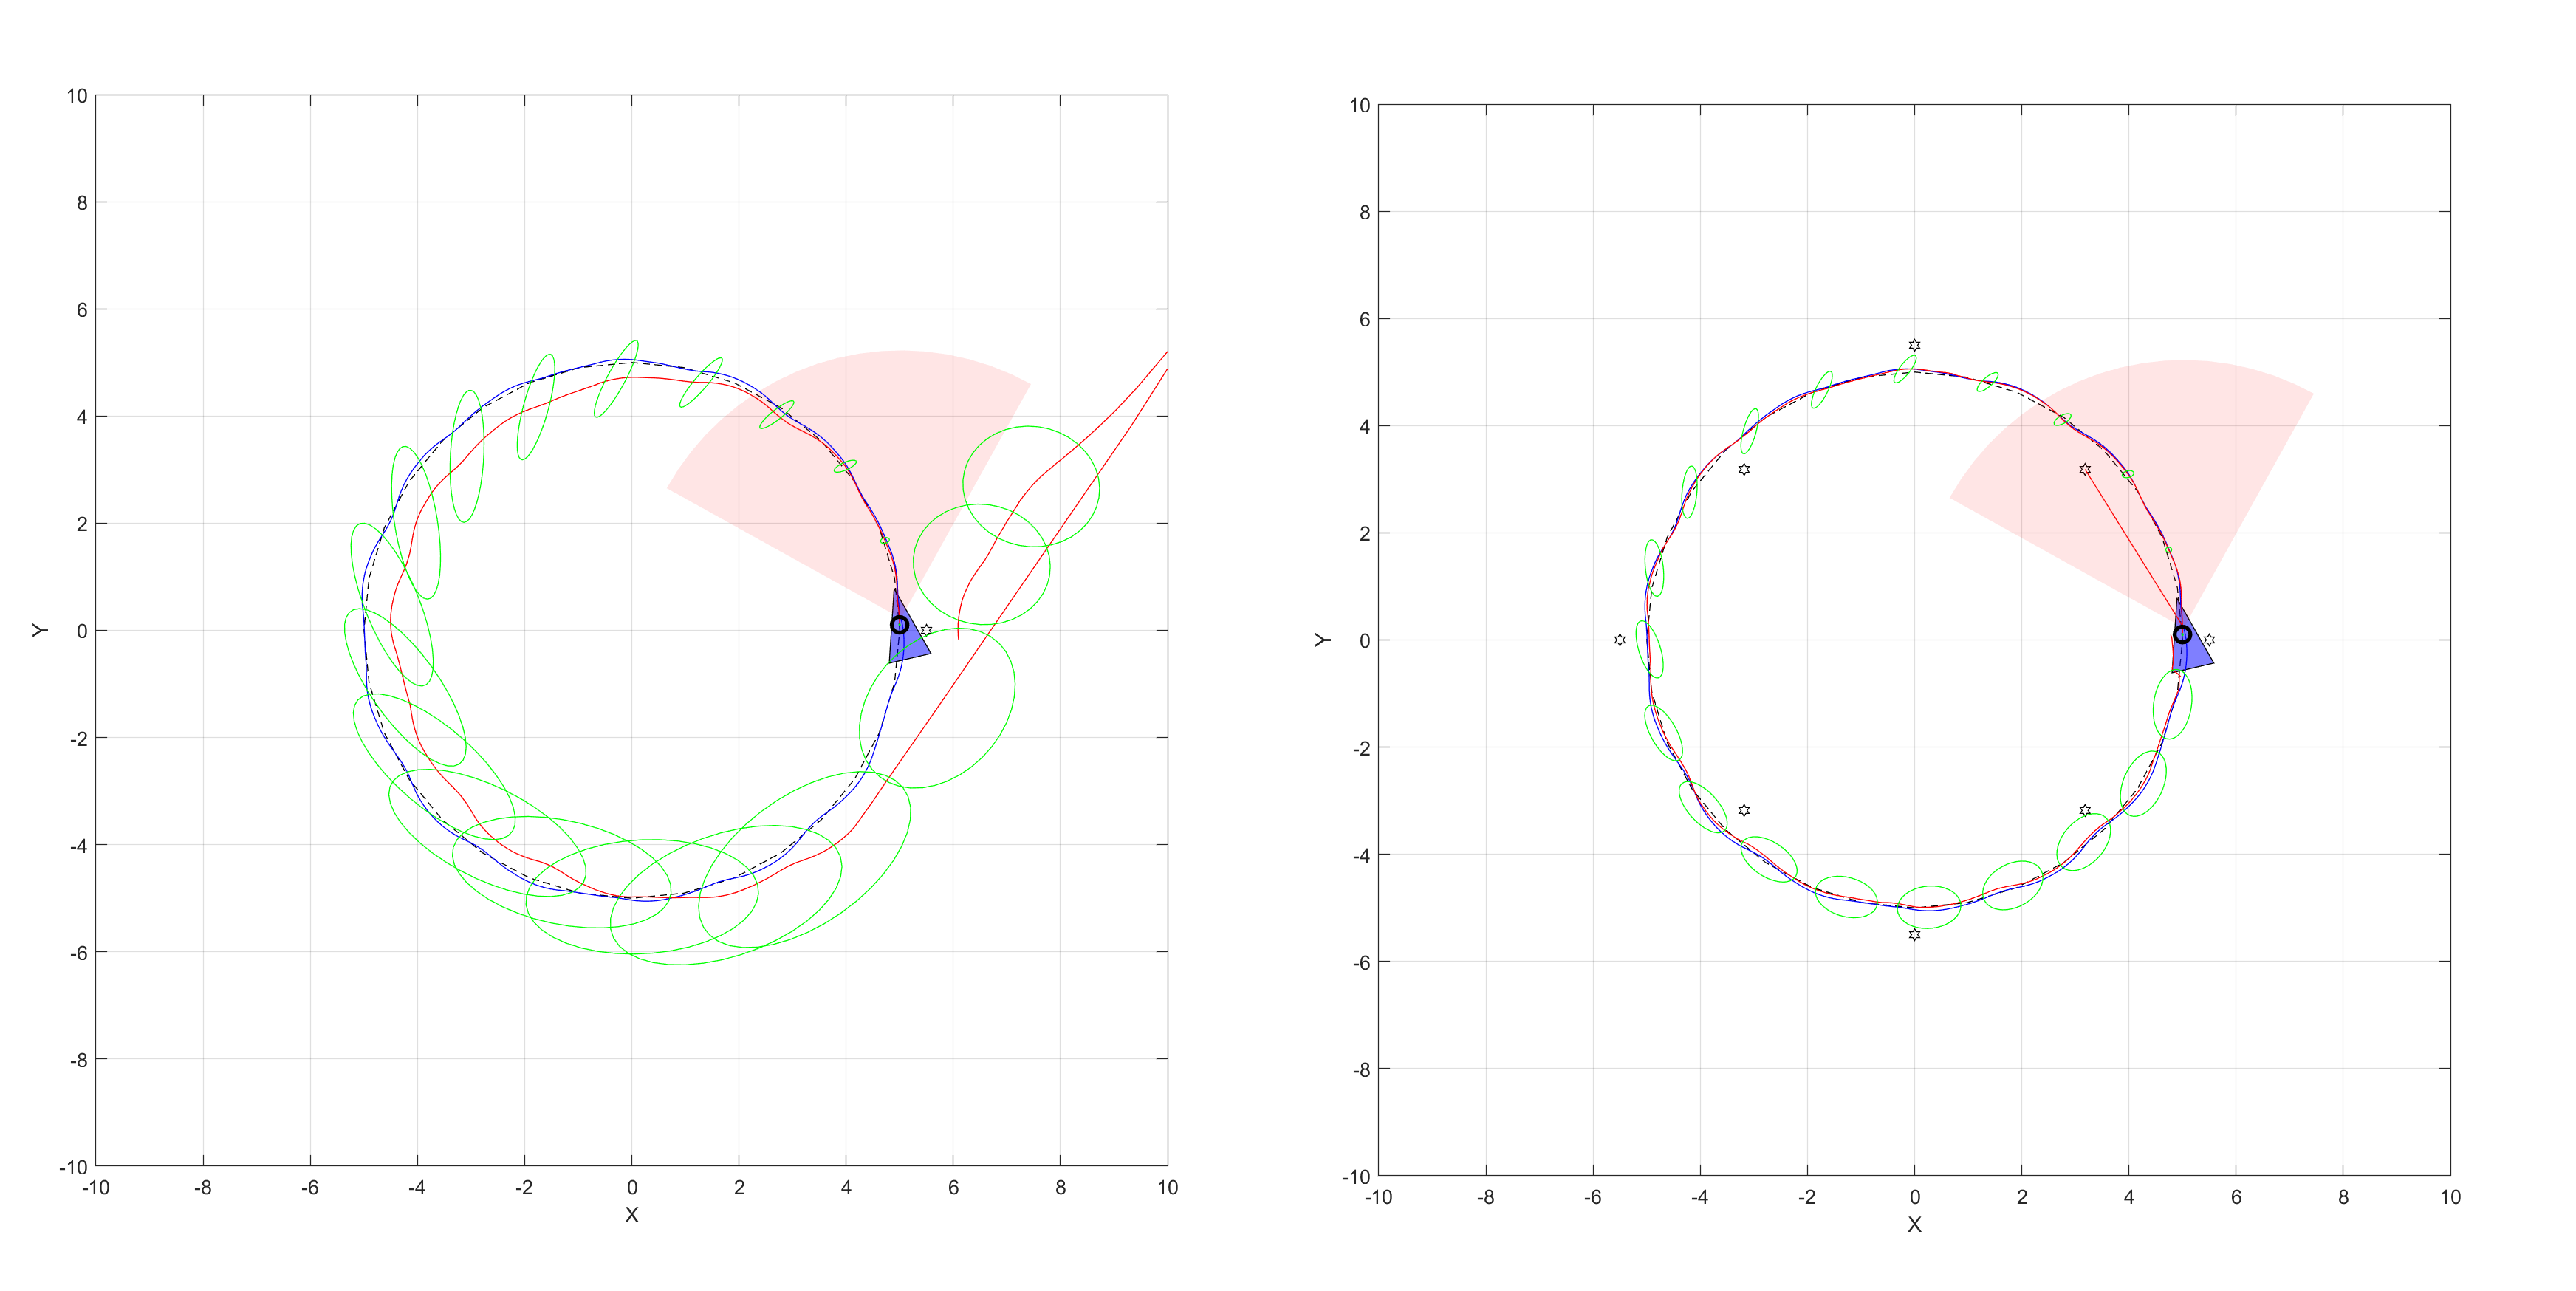
\includegraphics[width=.75\linewidth]{Figures/2.png}
%	\caption{Kreisfahrt nur mit Startmarker und extra Markern. Die eigentlich gefahrene Strecke ist blau dargestellt, die geschätzte Strecke rot. Die grünen Ellipsen umranden den $1\sigma$ Bereich der Positionsunsicherheit}
%	\label{fig:simulation}
%\end{figure}

Schon nach Umfahrung des halben Kurses nur mit Startmarker ist eine deutliche Abweichung der geschätzten Strecke zur eigentlichen zu erkennen. Warum die geschätzte Position bei Erreichen des Startmarkers den Kartenbereich verlässt, bedarf noch eine genauere Untersuchung.
\section{Massenträgheitsmoment}
\subsection{Theorie}
Das Trägheitsmoment kann experimentell durch einen Pendelversuch bestimmt werden. 
Für eine harmonische Schwingung kann die Auslenkung $x$ mit der Kreisfrequenz $\omega$ als Funktion der Zeit dargestellt werden:
\[ \frac{d^2x}{dt^2}+\omega^2x=0.\]
Das Drehmoment, das auf den Körper wirkt beträgt 
\[M=-mgd = -mglsin(\varphi).\]
In Verbindung mit \(M(t) = I\alpha(t)\) gilt \[ \frac{d^2\varphi}{dt^2}+\frac{mgl}{I}sin(\varphi)=0.\]
Für kleine Winkel und der damit verbundenen Annahme \(sin(\varphi)\approx \varphi\) gilt \[\frac{d^2\varphi}{dt^2}+\frac{mgl}{I} \varphi =0.\]
Damit ist  die Schwingungsdauer $T$  
\[T=\frac{2\pi}{\omega} = 2\pi \sqrt{\frac{I}{mgl}}\] 
und das Trägheitsmoment $I$ 
\[I=\Big(\frac{T}{2\pi}\Big)^2mgl.\]

\subsection{Praxisversuch}
Das für den Pendelversuch verwendete Pendel besteht aus einer Holzplatte und einem Gestell. Das kombinierte Trägheitsmoment für Platte und Gestell bezüglich des gemeinsamen Schwerpunktes beträgt $0,057 kg m^2.$
Die Schwingungsdauer $T$ mit montiertem Autos beträgt $1,3749s$, das Gesamtgewicht aus Holzplatte, Gestell und Auto ergibt sich zu $m_{ges}=0,846+1,152+2,26 = 4,258kg$. Die Pendellänge $l$ ist der Abstand  vom gemeinsamen Schwerpunkt zur Drehachse und beträgt  $0,383m.$   Daraus  ergibt sich ein Trägheitsmoment von 
\[I_{ges} = \Big(\frac{1,3749}{2\pi}\Big)^2 \cdot 4,258 \cdot 9.81 \cdot 0.383 = 0,7662 kg m^2.\]
Dieses ist das Trägheitsmoment  des kombinierten Körpers (Holzplatte, Gestell und Auto) bezüglich der Drehachse. Mit Hilfe des Steiner'schen Satzes kann die Bezugsachse in den gemeinsamen Schwerpunkt verschoben werden: 
\[I_{ges,SP} = I_{ges} + m_{ges} \cdot l^2  \hspace{5mm} \rightarrow  \hspace{5mm} 0,7662 + 4,258 \cdot 0,383^2 = 1,39kgm^2.\] 
Das Trägheitsmoment des Autos bezüglich des Schwerpunkts berechnet sich aus der Differenz des Gesamtträgheitsmoment und des Trägheitsmoment der Aufhängung:
\[1,39-0,057 = 1,333 kgm^2.\]
\section{Beziehung von Stellgrößen der Motoren zu Lenkwinkel und Geschwindigkeit}
\subsection{Geschwindigkeit}
Um die Geschwindigkeit zu einer jeweils vorgegebenen Leistung am Motor zu bestimmen, haben wir das Auto auf gerader Strecke durch zwei Lichtschranken fahren lassen. Mithilfe eines Osziloskops konnten wir die Kurvenverläufe an den Ausgängen der Lichtschranken vergleichen und so die Zeit bestimmen, die das Auto gebraucht hat um die Strecke zwischen den beiden Schranken zurück zu legen. Mit einem aufgeklebten Papier an der Fahrzeugfront haben wir sichergestellt, dass trotz leichter Höhendifferenzen bei beiden Lichtschranken die erste Flanke des Ausgangssignals der gleichen Lage des Autos relativ zur Schranke entspricht.

Bezeichne $x(t): [0,\infty]\rightarrow \mathbb{R}$ die Lage des Autos in Fahrtrichtung, $l\in[0,\infty]$ den Abstand zwischen den beiden Lichtschranken und $t_1, t_2\in [0,\infty]$ den Zeitpunkt, bei dem die Fahrzeugfront an der ersten, beziehungsweise zweiten Lichtschranke ist. Dann lässt sich die Durschnittsgeschwindigkeit $v_d\in\mathbb{R}$ des Autos zwischen den beiden Schranken folgendermaßen berechnen:
\begin{equation*}
v_d := \frac{\int_{t_0}^{t_1}{\dot x(t) dt}}{t_1-t_0}=\frac{x(t_1)-x(t_2)}{t_1-t_0}=\frac{l}{t_1-t_0}
\end{equation*}
Wenn wir sicherstellen, dass das Auto zwischen den Schranken eine konstante Geschwindigkeit $v\in\mathbb{R}$ fährt, also $\dot x\vert_{t\in[t_0,t_1]}\equiv v$, entspricht $v_d=v$:
\begin{equation*}
v_d = \frac{\int_{t_0}^{t_1}{\dot x(t) dt}}{t_1-t_0} = \frac{\int_{t_0}^{t_1}{v dt}}{t_1-t_0}=v\frac{t_1-t_0}{t_1-t_0}=v
\end{equation*}
Falls die angenommenen Länge um $\Delta l\in\mathbb{R}$ von der wirklichen Länge $l$ abweicht, ergibt sich ein Fehler $e\in \mathbb{R}$ bei der Bestimmung der Geschwindigkeit von
\begin{equation*}
	e = \frac{\Delta l}{t_1-t_0} = \frac{\Delta l}{\frac{l}{v}} = \frac{\Delta l}{l}v.
\end{equation*}

Wir gehen davon aus, dass wir die Lichtschranken im Abstand von $1m\pm1cm$ genau plaziert haben, also deshalb die Geschwindigkeit bis auf $1\%$ genau bestimmen konnten. Den Messfehler bei der Zeitmessung betrachten wir hier nicht, da er sich mit dem Oszilloskop bis auf Millisekunden sehr genau bestimmen ließ. Die Messergebnisse sind in Abbildung~\ref{fig:motor_speed} dargestellt.

\begin{figure}
\begin{subfigure}{.5\textwidth}
	\centering
	% This file was created by matlab2tikz.
%
%The latest updates can be retrieved from
%  http://www.mathworks.com/matlabcentral/fileexchange/22022-matlab2tikz-matlab2tikz
%where you can also make suggestions and rate matlab2tikz.
%
\definecolor{mycolor1}{rgb}{0.00000,0.44700,0.74100}%
%
\begin{tikzpicture}

\begin{axis}[%
width=0.5\textwidth,
height=0.8\textwidth,
at={(0.758in,0.481in)},
scale only axis,
xmin=0,
xmax=30,
xlabel style={font=\color{white!15!black}},
xlabel={$\times 100$ Motor Speed},
ymin=0.2,
ymax=1.8,
ylabel style={font=\color{white!15!black}},
ylabel={$v$ in $m/s$},
axis background/.style={fill=white},
xmajorgrids,
ymajorgrids
]
\addplot [color=mycolor1, mark=asterisk, mark options={solid, mycolor1}, forget plot]
  table[row sep=crcr]{%
3.5	0.378931413414172\\
4	0.419991600167997\\
5	0.562429696287964\\
10	0.987166831194472\\
15	1.26262626262626\\
20	1.46198830409357\\
25	1.5625\\
30	1.67224080267559\\
};
\end{axis}
\end{tikzpicture}%
	\caption[Motor Speed]{Geschwindigkeit}
	\label{fig:motor_speed}
\end{subfigure}
\begin{subfigure}{.5\textwidth}
	\centering
	% This file was created by matlab2tikz.
%
%The latest updates can be retrieved from
%  http://www.mathworks.com/matlabcentral/fileexchange/22022-matlab2tikz-matlab2tikz
%where you can also make suggestions and rate matlab2tikz.
%
\definecolor{mycolor1}{rgb}{0.00000,0.44700,0.74100}%
%
\begin{tikzpicture}

\begin{axis}[%
width=0.5\textwidth,
height=0.8\textwidth,
at={(0.758in,0.481in)},
scale only axis,
xmin=-3,
xmax=3,
xlabel style={font=\color{white!15!black}},
xlabel={$\times 100$ Motor Angle},
ymin=-25,
ymax=20,
ylabel style={font=\color{white!15!black}},
ylabel={Radwinkel in $^\circ$},
axis background/.style={fill=white},
xmajorgrids,
ymajorgrids
]
\addplot [color=mycolor1, mark=asterisk, mark options={solid, mycolor1}, forget plot]
  table[row sep=crcr]{%
-3	-25\\
-2	-20\\
-1	-12\\
0	0\\
1	7\\
2	14.2\\
3	20\\
};
\end{axis}
\end{tikzpicture}%
	\caption[Motor Angle]{Lenkwinkel}
	\label{fig:motor_angle}
\end{subfigure}
\caption[Simulink Stellgrößen]{Messergebnisse für die Simulink Stellgrößen \texttt{Motor Speed}~(\ref{fig:motor_speed}) und \texttt{Motor Angle}~(\ref{fig:motor_angle})}
\end{figure}


\subsection{Lenkwinkel}

Um den Lenkwinkel zu messen, haben wir die Reifenstellung auf ein Papier abgetragen und die jeweiligen Winkel mit dem Geodreieck gemessen. Aufgrund von Fehlern beim Abtragen sowie dem recht großen Spiel der Reifen bei fest gesetzten Lenkwinkel schätzen wir den Messfehler auf $\pm5^\circ$ ein. Aus den Messergebnissen in Abbildung~\ref{fig:motor_angle} kann man einen linearen Zusammenhang erahnen.

\section{Über-/Untersteuerung und Seitenkraftbeiwerte}
\subsection{Über-/Untersteuerung}
Ob das Auto über- oder untersteuert, kann bei einer Kreisfahrt  untersucht werden. Wir haben festgestellt, dass sich der Radius des Kreises, auf dem sich das Auto bewegt, beim Erhöhen der Geschwindigkeit vergrößert. Dies spricht für ein \textbf{Untersteuern} des Fahrzeuges.

\subsection{Seitenkraftbeiwerte}

Um die Seitenkraftbeiwerte abzuschätzen, haben wir eine Keisfahrt mit konstanter Geschwindigkeit $v=1.66\frac{m}{s}$ auf einem Kreis mit Radius $R=0.84m$ durchgeführt. Der gemittelte Vorderradwinkel betrug $\delta_V=22.5^\circ$. Bei einer solchen Kreisfahrt ist die zweite Ableitung der Gierrate $\ddot{\Psi}$ und die erste Ableitung des Schwimmwinkels $ \beta$ null. Außerdem ist $\dot{\Psi}=\frac{v}{R}$ und $\beta$ konstant. Wenn man nun noch zusätzlich annimmt, dass $S_L=M_{LZ}=0$ gilt, vereinfacht sich die lineare Bewegungsgleichung
$$ \begin{bmatrix} 
mv^2 & 0 \\
0 & I 
\end{bmatrix} 
\begin{bmatrix} 
\dot{\beta} \\
\ddot{\Psi}
\end{bmatrix}+ 
\begin{bmatrix} 
mv+k_{SV}l_V-k_{SH}l_{H} \\
\frac{k_{SV}l_V^2+k_{SH}l_H^2}{v}  
\end{bmatrix} \dot{\Psi}+
\begin{bmatrix} 
k_{SV}+k_{SH} \\
k_{SV}l_V-k_{SH}l_H 
\end{bmatrix} \beta=
\begin{bmatrix} 
S_L+k_{SV}\delta_v \\
M_{LZ}+k_{SV}l_V\delta_V 
\end{bmatrix}
$$
auf 
$$  
\begin{bmatrix} 
mv+k_{SV}l_V-k_{SH}l_{H} \\
\frac{k_{SV}l_V^2+k_{SH}l_H^2}{v}  
\end{bmatrix} \frac{v}{R}+
\begin{bmatrix} 
k_{SV}+k_{SH} \\
k_{SV}l_V-k_{SH}l_H 
\end{bmatrix} \beta=
\begin{bmatrix} 
k_{SV}\delta_V \\
k_{SV}l_V\delta_V 
\end{bmatrix}.
$$

Wenn man diese nach $K_{SH}$ beziehungsweise $K_{SV}$ umstellt, erhält man 
$$
K_{SH}=\frac{l_V mv^2}{l(l_H-R\beta)} \qquad \qquad K_{SV}=\frac{l_H}{l^2\frac{R\delta_V-l}{mlv^2}+\frac{l_V}{K_{SH}}}.
$$

Aus vorherigen Versuchen sind folgende Parameter bekannt:

$m=2.2061 kg,l_V=0.1421 m,l_H=0.1195 m,l=0.261 m$. Um $K_{SH}$ zu bestimmen wird nun also nur noch der Schwimmwinkel benötigt. 



Da dieser sehr klein ist und das Auto auf den Aufnahmen der Kreisfahrt nicht sonderlich scharf ist, ist es nicht einfach diesen exakt zu messen. Um eine grobe Idee zu bekommen, wo er liegen könnte, kann man eine Tangente (rot) des Kreises betrachten, auf dem das Auto sich bewegt. Auf dieser Tangente liegt der Geschwindigkeitsvektor $v$ des Autos. Die blaue Linie zeigt in die Richtung, in die das Auto zeigt. Der Schwimmwinkel ist nun der Winkel zwischen diesen beiden Linien. 

Abhängig vom tatsächlichen $\beta$ ergibt sich, wobei Fehler in den anderen Parametern vernachlässigt werden, da deren Einfluss dessen Fehler auf die Seitenkraftbeiwerte im Vergleich zum Fehler von $\beta$ klein sind:\\
\begin{center}
\begin{tabular}{|c|c|c|c|}
\hline
$\beta$ in Grad & $k_{SH}$& $k_{SV}$&$k_{SH}l_H-k_{SV}l_V$ \\\hline

-1  & 22.61 & 12.96&0.86\\\hline
0  & 28.18 & 14.97&1.24\\\hline
1  & 32.14 & 16.24&1.53\\\hline
2  & 37.39 & 17.73&1.95\\\hline
3  & 44.70 & 19.53&2.57\\\hline
4  & 55.56 & 21.74&3.55\\\hline
4.4  & 61.54 & 22.77&4.12\\\hline
5  & 73.38 & 24.51&5.29\\\hline

\end{tabular}\\
\end{center}
Somit sind Seitenkraftbeiwerte mit $28<k_{SH}<75$ und $15<k_{SV}<25$ denkbar. Da $k_{SH}l_H-k_{SV}l_V$ in jedem Fall positiv ist, spricht dies auch für ein Untersteuern des Fahrzeuges.
\begin{center}
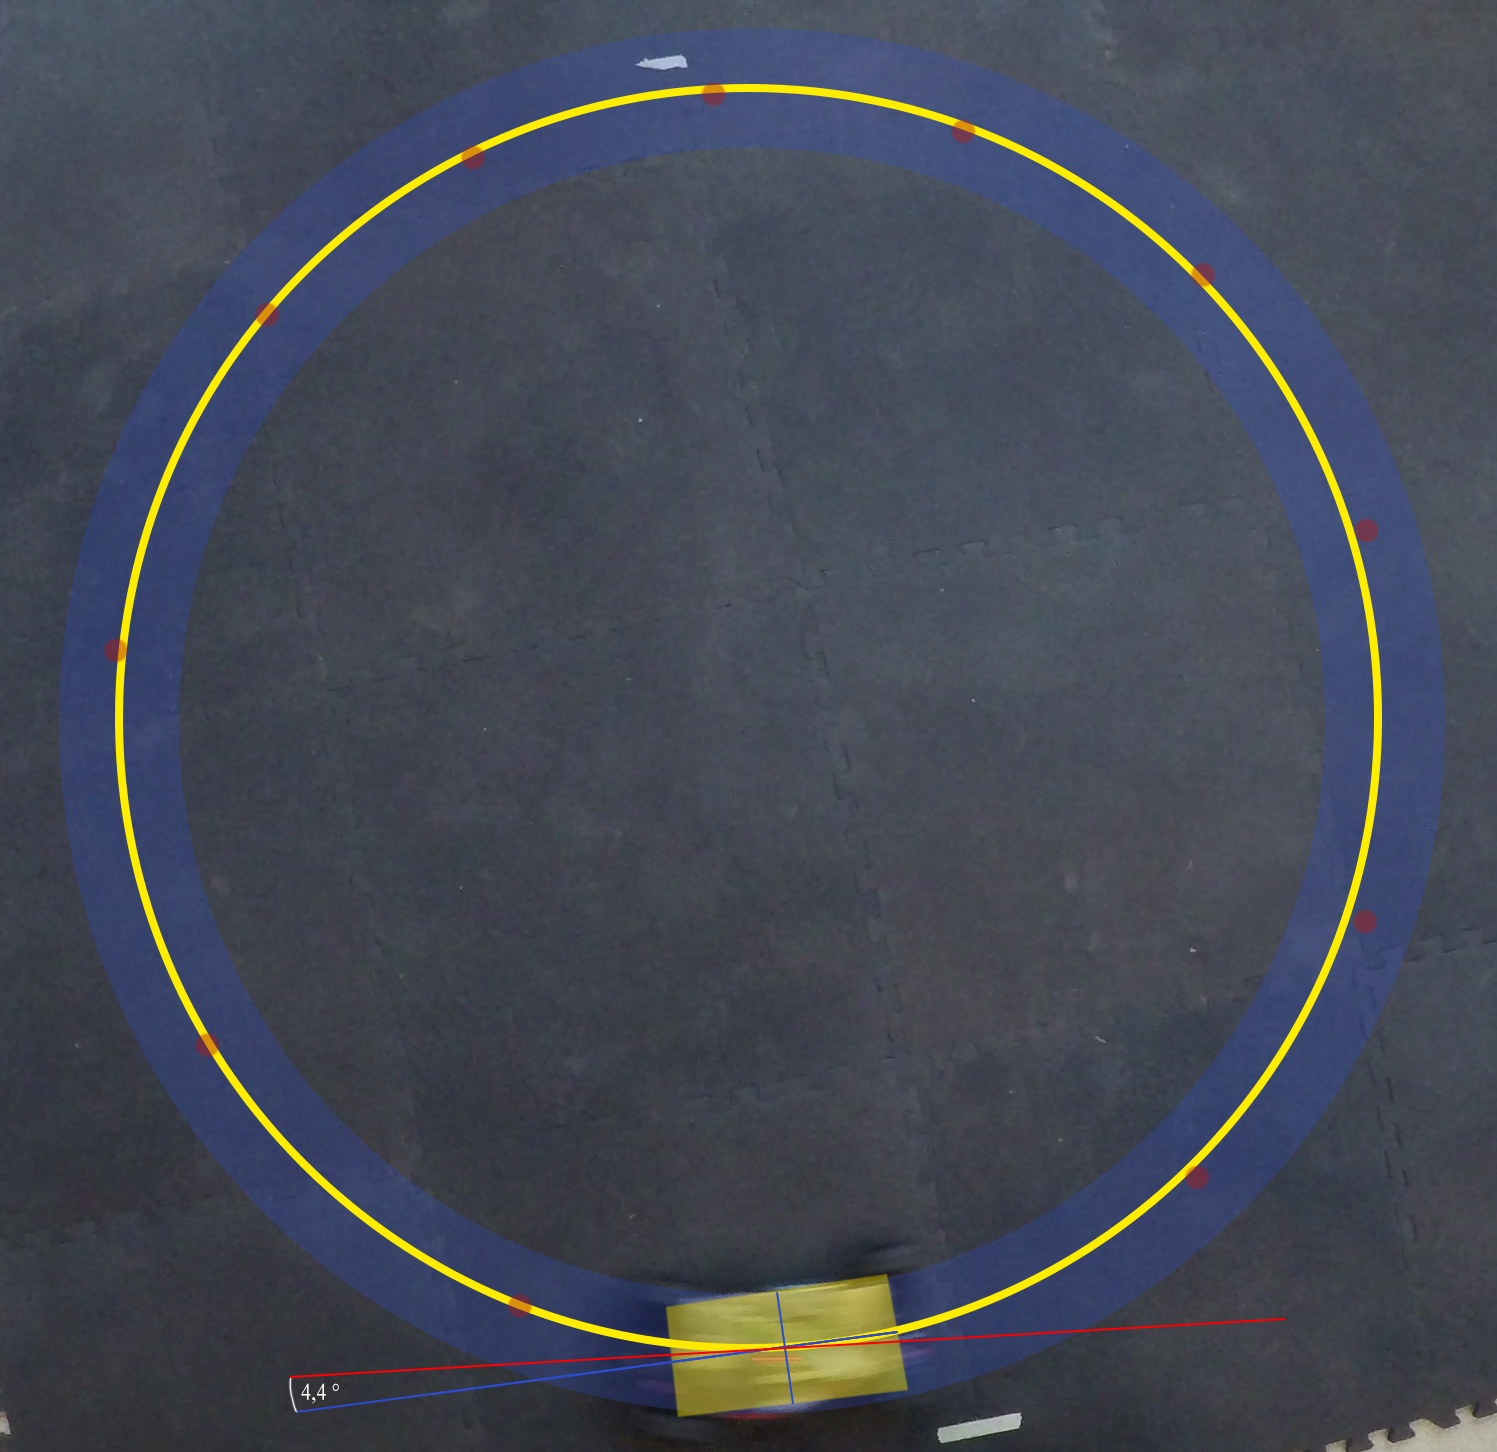
\includegraphics[scale=0.2]{Figures/Schwimmwinkel.png}\\

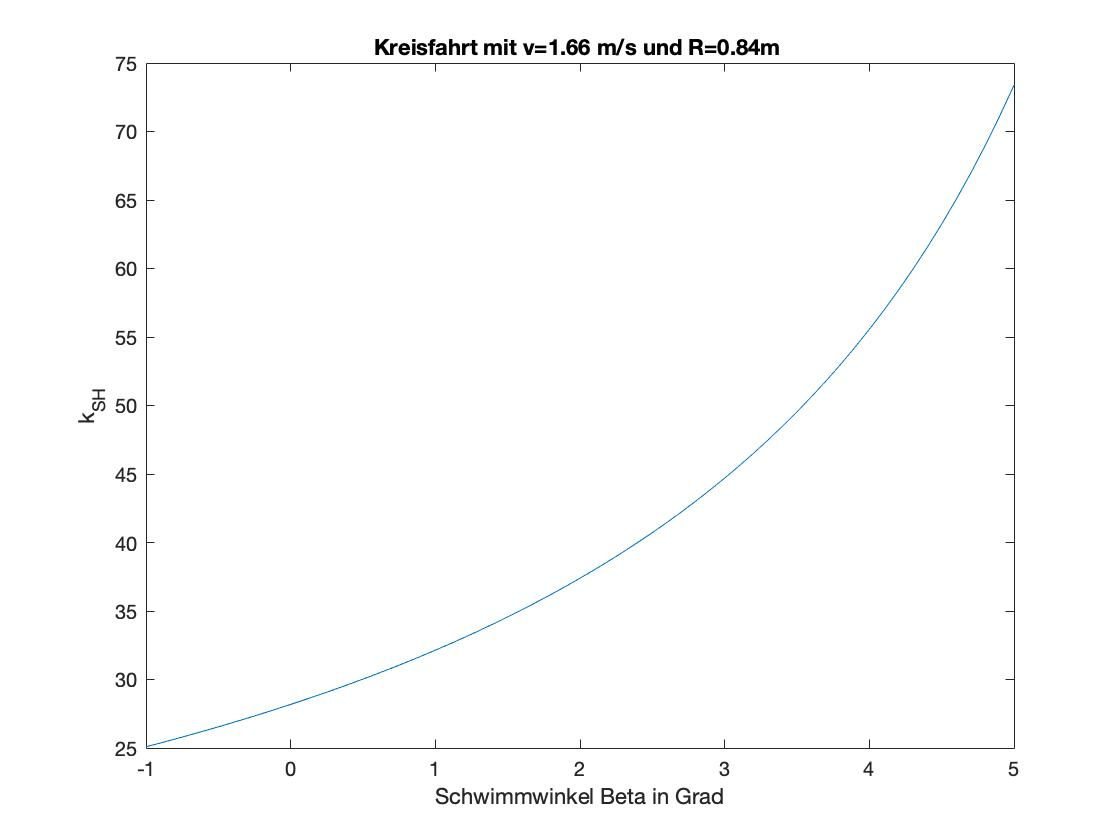
\includegraphics[scale=0.3]{Figures/ksh(beta).jpg}\\

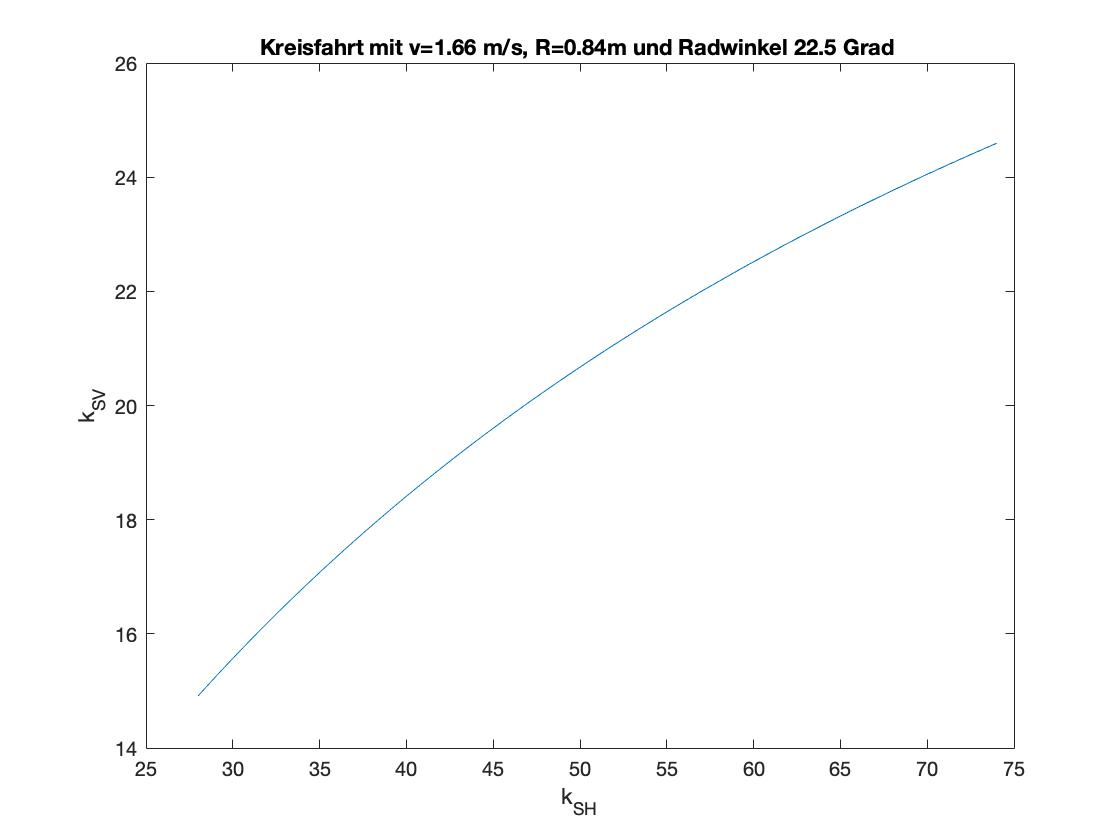
\includegraphics[scale=0.3]{Figures/ksv(ksv).jpg}
\end{center}


\end{document}